 \let\negmedspace\undefined
\let\negthickspace\undefined
\documentclass[journal]{IEEEtran}
\usepackage[a5paper, margin=10mm, onecolumn]{geometry}
%\usepackage{lmodern} % Ensure lmodern is loaded for pdflatex
\usepackage{tfrupee} % Include tfrupee package

\setlength{\headheight}{1cm} % Set the height of the header box
\setlength{\headsep}{0mm}     % Set the distance between the header box and the top of the text
\usepackage{gvv-book}
\usepackage{gvv}
\usepackage{cite}
\usepackage{amsmath,amssymb,amsfonts,amsthm}
\usepackage{algorithmic}
\usepackage{graphicx}
\usepackage{textcomp}
\usepackage{xcolor}
\usepackage{txfonts}
\usepackage{listings}
\usepackage{enumitem}
\usepackage{mathtools}
\usepackage{gensymb}
\usepackage{comment}
\usepackage[breaklinks=true]{hyperref}
\usepackage{tkz-euclide} 
\usepackage{listings}
% \usepackage{gvv}                                        
\def\inputGnumericTable{}                                 
\usepackage[latin1]{inputenc}                                
\usepackage{color}                                            
\usepackage{array}                                            
\usepackage{longtable}                                       
\usepackage{calc}                                             
\usepackage{multirow}                                         
\usepackage{hhline}                                           
\usepackage{ifthen}                                           
\usepackage{lscape}



\usepackage{amsmath,amssymb}
\usepackage{booktabs}
\usepackage{tikz}
\usetikzlibrary{arrows.meta,angles,quotes}





\begin{document}

\bibliographystyle{IEEEtran}
\vspace{3cm}

\title{4.4.17}
\author{AI25BTECH11021 - Abhiram Reddy N}
% \maketitle
% \newpage
% \bigskip
{\let\newpage\relax\maketitle}

\renewcommand{\thefigure}{\theenumi}
\renewcommand{\thetable}{\theenumi}
\setlength{\intextsep}{10pt} % Space between text and floats


\numberwithin{equation}{enumi}
\numberwithin{figure}{enumi}
\renewcommand{\thetable}{\theenumi}


\section*{\textbf{Question}}
A point \(\mathbf{P}\) divides the line segment joining the points \(\mathbf{A}(3, -5)\) and \(\mathbf{B}(-4, 8)\) such that \(\frac{AP}{PB} = \frac{K}{1}\). If \(\mathbf{P}\) lies on the line \(x + y = 0\), then find the value of \(K\).

\section*{\textbf{Answer}}

\subsection*{\textbf{Step 1: Represent points as column vectors}}
\[
\mathbf{A} = \begin{pmatrix} a_1 \\ a_2 \end{pmatrix}, \quad 
\mathbf{B} = \begin{pmatrix} b_1 \\ b_2 \end{pmatrix}.
\]

\subsection*{\textbf{Step 2: Express \(\mathbf{P}\) using section formula in vector form}}
Since \(\mathbf{P}\) divides \(\mathbf{AB}\) in the ratio \(K : 1\), 
\[
\mathbf{P} = \frac{K \mathbf{B} + \mathbf{A}}{K + 1}.
\]

\subsection*{\textbf{Step 3: Use the line equation condition}}
Suppose the line is given as
\[
\mathbf{n}^\top \mathbf{x} = c, \quad \text{where } \mathbf{n} = \begin{pmatrix} n_1 \\ n_2 \end{pmatrix}.
\]
Since \(\mathbf{P}\) lies on this line,
\[
\mathbf{n}^\top \mathbf{P} = c.
\]
Substitute for \(\mathbf{P}\):
\[
\mathbf{n}^\top \left(\frac{K\mathbf{B} + \mathbf{A}}{K+1}\right) = c.
\]

\subsection*{\textbf{Step 4: Derive general formula for \(K\)}}
Multiplying through,
\[
\mathbf{n}^\top (K\mathbf{B} + \mathbf{A}) = c(K+1).
\]
\[
K(\mathbf{n}^\top \mathbf{B} - c) = c - \mathbf{n}^\top \mathbf{A}.
\]
\[
K = \frac{c - \mathbf{n}^\top \mathbf{A}}{\mathbf{n}^\top \mathbf{B} - c}.
\]

\subsection*{\textbf{Step 5: Substitute given values}}
Here,
\[
\mathbf{A} = \begin{pmatrix} 3 \\ -5 \end{pmatrix}, \quad 
\mathbf{B} = \begin{pmatrix} -4 \\ 8 \end{pmatrix}, \quad 
\mathbf{n} = \begin{pmatrix} 1 \\ 1 \end{pmatrix}, \quad 
c = 0.
\]
Thus,
\[
K = \frac{0 - (1\cdot 3 + 1\cdot (-5))}{(1\cdot (-4) + 1\cdot 8) - 0}
= \frac{-(-2)}{4}
= \frac{2}{4}
= \frac{1}{2}.
\]

\subsection*{\textbf{Final answer}}
\[
\boxed{K = \tfrac{1}{2}}
\]

\begin{figure}[htbp]
\centering
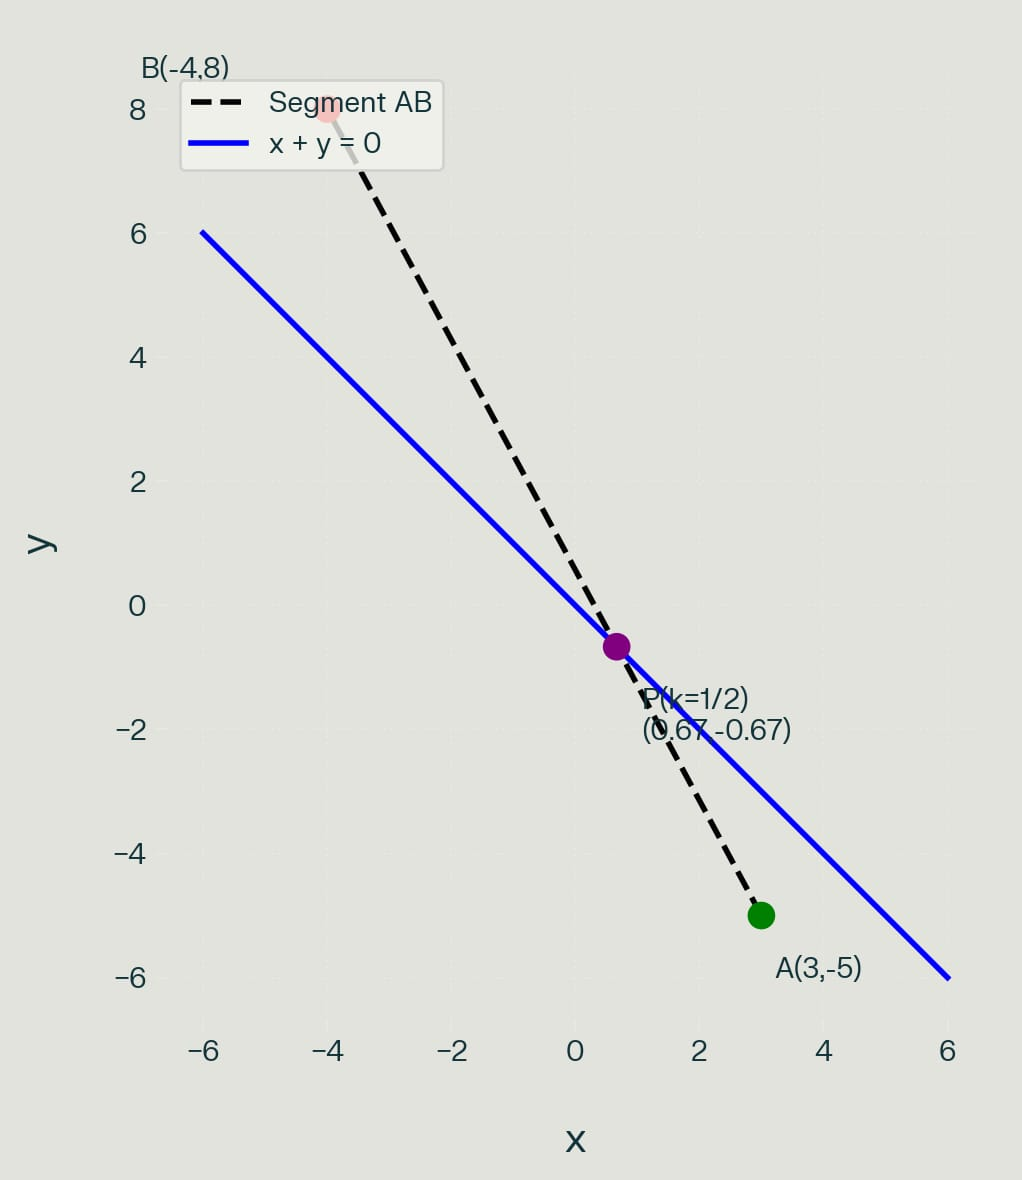
\includegraphics[width=0.7\columnwidth]{figs/python_plot.png} 
\caption{Plot of the points and line showing the division ratio.}
\label{fig:1}
\end{figure}


\end{document}
